% Options for packages loaded elsewhere
\PassOptionsToPackage{unicode}{hyperref}
\PassOptionsToPackage{hyphens}{url}
\PassOptionsToPackage{dvipsnames,svgnames,x11names}{xcolor}
%
\documentclass[
]{memoir}
\usepackage{amsmath,amssymb}
\usepackage{lmodern}
\usepackage{iftex}
\ifPDFTeX
  \usepackage[T1]{fontenc}
  \usepackage[utf8]{inputenc}
  \usepackage{textcomp} % provide euro and other symbols
\else % if luatex or xetex
  \usepackage{unicode-math}
  \defaultfontfeatures{Scale=MatchLowercase}
  \defaultfontfeatures[\rmfamily]{Ligatures=TeX,Scale=1}
  \setmonofont[]{Inconsolata}
\fi
% Use upquote if available, for straight quotes in verbatim environments
\IfFileExists{upquote.sty}{\usepackage{upquote}}{}
\IfFileExists{microtype.sty}{% use microtype if available
  \usepackage[]{microtype}
  \UseMicrotypeSet[protrusion]{basicmath} % disable protrusion for tt fonts
}{}
\makeatletter
\@ifundefined{KOMAClassName}{% if non-KOMA class
  \IfFileExists{parskip.sty}{%
    \usepackage{parskip}
  }{% else
    \setlength{\parindent}{0pt}
    \setlength{\parskip}{6pt plus 2pt minus 1pt}}
}{% if KOMA class
  \KOMAoptions{parskip=half}}
\makeatother
\usepackage{xcolor}
\IfFileExists{xurl.sty}{\usepackage{xurl}}{} % add URL line breaks if available
\IfFileExists{bookmark.sty}{\usepackage{bookmark}}{\usepackage{hyperref}}
\hypersetup{
  pdftitle={Data Science per psicologi},
  pdfauthor={Corrado Caudek},
  colorlinks=true,
  linkcolor={Maroon},
  filecolor={Maroon},
  citecolor={Blue},
  urlcolor={Blue},
  pdfcreator={LaTeX via pandoc}}
\urlstyle{same} % disable monospaced font for URLs
\usepackage{color}
\usepackage{fancyvrb}
\newcommand{\VerbBar}{|}
\newcommand{\VERB}{\Verb[commandchars=\\\{\}]}
\DefineVerbatimEnvironment{Highlighting}{Verbatim}{commandchars=\\\{\}}
% Add ',fontsize=\small' for more characters per line
\usepackage{framed}
\definecolor{shadecolor}{RGB}{248,248,248}
\newenvironment{Shaded}{\begin{snugshade}}{\end{snugshade}}
\newcommand{\AlertTok}[1]{\textcolor[rgb]{0.94,0.16,0.16}{#1}}
\newcommand{\AnnotationTok}[1]{\textcolor[rgb]{0.56,0.35,0.01}{\textbf{\textit{#1}}}}
\newcommand{\AttributeTok}[1]{\textcolor[rgb]{0.77,0.63,0.00}{#1}}
\newcommand{\BaseNTok}[1]{\textcolor[rgb]{0.00,0.00,0.81}{#1}}
\newcommand{\BuiltInTok}[1]{#1}
\newcommand{\CharTok}[1]{\textcolor[rgb]{0.31,0.60,0.02}{#1}}
\newcommand{\CommentTok}[1]{\textcolor[rgb]{0.56,0.35,0.01}{\textit{#1}}}
\newcommand{\CommentVarTok}[1]{\textcolor[rgb]{0.56,0.35,0.01}{\textbf{\textit{#1}}}}
\newcommand{\ConstantTok}[1]{\textcolor[rgb]{0.00,0.00,0.00}{#1}}
\newcommand{\ControlFlowTok}[1]{\textcolor[rgb]{0.13,0.29,0.53}{\textbf{#1}}}
\newcommand{\DataTypeTok}[1]{\textcolor[rgb]{0.13,0.29,0.53}{#1}}
\newcommand{\DecValTok}[1]{\textcolor[rgb]{0.00,0.00,0.81}{#1}}
\newcommand{\DocumentationTok}[1]{\textcolor[rgb]{0.56,0.35,0.01}{\textbf{\textit{#1}}}}
\newcommand{\ErrorTok}[1]{\textcolor[rgb]{0.64,0.00,0.00}{\textbf{#1}}}
\newcommand{\ExtensionTok}[1]{#1}
\newcommand{\FloatTok}[1]{\textcolor[rgb]{0.00,0.00,0.81}{#1}}
\newcommand{\FunctionTok}[1]{\textcolor[rgb]{0.00,0.00,0.00}{#1}}
\newcommand{\ImportTok}[1]{#1}
\newcommand{\InformationTok}[1]{\textcolor[rgb]{0.56,0.35,0.01}{\textbf{\textit{#1}}}}
\newcommand{\KeywordTok}[1]{\textcolor[rgb]{0.13,0.29,0.53}{\textbf{#1}}}
\newcommand{\NormalTok}[1]{#1}
\newcommand{\OperatorTok}[1]{\textcolor[rgb]{0.81,0.36,0.00}{\textbf{#1}}}
\newcommand{\OtherTok}[1]{\textcolor[rgb]{0.56,0.35,0.01}{#1}}
\newcommand{\PreprocessorTok}[1]{\textcolor[rgb]{0.56,0.35,0.01}{\textit{#1}}}
\newcommand{\RegionMarkerTok}[1]{#1}
\newcommand{\SpecialCharTok}[1]{\textcolor[rgb]{0.00,0.00,0.00}{#1}}
\newcommand{\SpecialStringTok}[1]{\textcolor[rgb]{0.31,0.60,0.02}{#1}}
\newcommand{\StringTok}[1]{\textcolor[rgb]{0.31,0.60,0.02}{#1}}
\newcommand{\VariableTok}[1]{\textcolor[rgb]{0.00,0.00,0.00}{#1}}
\newcommand{\VerbatimStringTok}[1]{\textcolor[rgb]{0.31,0.60,0.02}{#1}}
\newcommand{\WarningTok}[1]{\textcolor[rgb]{0.56,0.35,0.01}{\textbf{\textit{#1}}}}
\usepackage{longtable,booktabs,array}
\usepackage{calc} % for calculating minipage widths
% Correct order of tables after \paragraph or \subparagraph
\usepackage{etoolbox}
\makeatletter
\patchcmd\longtable{\par}{\if@noskipsec\mbox{}\fi\par}{}{}
\makeatother
% Allow footnotes in longtable head/foot
\IfFileExists{footnotehyper.sty}{\usepackage{footnotehyper}}{\usepackage{footnote}}
\makesavenoteenv{longtable}
\usepackage{graphicx}
\makeatletter
\def\maxwidth{\ifdim\Gin@nat@width>\linewidth\linewidth\else\Gin@nat@width\fi}
\def\maxheight{\ifdim\Gin@nat@height>\textheight\textheight\else\Gin@nat@height\fi}
\makeatother
% Scale images if necessary, so that they will not overflow the page
% margins by default, and it is still possible to overwrite the defaults
% using explicit options in \includegraphics[width, height, ...]{}
\setkeys{Gin}{width=\maxwidth,height=\maxheight,keepaspectratio}
% Set default figure placement to htbp
\makeatletter
\def\fps@figure{htbp}
\makeatother
\setlength{\emergencystretch}{3em} % prevent overfull lines
\providecommand{\tightlist}{%
  \setlength{\itemsep}{0pt}\setlength{\parskip}{0pt}}
\setcounter{secnumdepth}{5}
\chapterstyle{bianchi}

\usepackage{mathtools}
\usepackage[italian]{babel} 
\usepackage{booktabs}
\usepackage{hyperref}
\hypersetup{
  colorlinks=true
}
\usepackage[
  labelfont=bf, 
  font={small, it} 
]{caption} 
\usepackage{upquote} % print correct quotes in verbatim-environments
\usepackage[autostyle, italian=quotes]{csquotes}
\usepackage{empheq} 
\usepackage{xfrac}

\raggedbottom % allow variable (ragged) site heights
\frenchspacing
% \setlength\parskip{1.5pt plus 1pt minus 0.5pt}

\DeclareMathOperator{\Var}{Var} % Define variance operator
\DeclareMathOperator{\SD}{SD} % Define sd operator
\DeclareMathOperator{\Cov}{Cov} % Define covariance operator
\DeclareMathOperator{\Corr}{Corr} % Define correlation operator
\DeclareMathOperator{\Me}{Me} % Define mediane operator
\DeclareMathOperator{\Mo}{Mo} % Define mode operator
\DeclareMathOperator{\Bin}{Bin} % Define binomial operator
\DeclareMathOperator{\Bernoulli}{Bernoulli} % Define Bernoulli operator
\DeclareMathOperator{\Poi}{Poi} % Define Poisson operator
\DeclareMathOperator{\Uniform}{Uniform} % Define Uniform operator
\DeclareMathOperator{\Cauchy}{Cauchy} % Define Cauchy operator
\DeclareMathOperator{\elpd}{elpd} % Define elpd operator
\DeclareMathOperator{\lppd}{lppd} % Define lppd operator
\DeclareMathOperator{\LOO}{LOO} % Define LOO operator
\DeclareMathOperator{\B}{\mathscr{B}} % Define Bernoulli operator
\newcommand{\R}{\textsf{R}} % Define R programming language symbol
\newcommand{\E}{\mathbb{E}} % Define expected value operator
\newcommand{\Real}{\mathbb{R}} % Define real number operator
\newcommand{\Prob}{\mathscr{P}}
\DeclareMathOperator*{\argmin}{arg\,min} % thin space, limits on side in displays
\DeclareMathOperator*{\argmax}{arg\,max} % thin space, limits on side in displays

\usepackage{microtype}

\ifLuaTeX
  \usepackage{selnolig}  % disable illegal ligatures
\fi
\usepackage[]{natbib}
\bibliographystyle{apalike}

\title{Data Science per psicologi}
\author{Corrado Caudek}
\date{2021-10-10}

\begin{document}
\maketitle

{
\hypersetup{linkcolor=}
\setcounter{tocdepth}{1}
\tableofcontents
}
\newpage

\vspace*{5cm}

\thispagestyle{empty}

\hypertarget{mod-binom}{%
\chapter{Modello Beta-Binomiale}\label{mod-binom}}

\hypertarget{una-proporzione}{%
\section{Una proporzione}\label{una-proporzione}}

Si considerino \(n\) variabili casuali Bernoulliane i.i.d.:
\[
y = (y_1, \dots, y_n) \stackrel{iid}{\sim} \mathcal{B}(\theta).
\]
\noindent
Vogliamo stimare \(\theta\) avendo osservato \(y\). Essendo i.i.d., i dati possono essere riassunti dal numero totale di successi nelle \(n\) prove, denotato da \(y\). Il modello binomiale è
\begin{equation}
p(y \mid \theta) = \Bin(y \mid n, \theta) = \binom{n}{y}\theta^y (1 -\theta)^{n-y},
\end{equation}
\noindent
dove nel termine di sinistra dell'equazione abbiamo ignorato \(n\) in quanto viene considerato fisso per disegno.

L'inferenza sul modello binomiale richiede di assegnare una distribuzione a priori su \(\theta\) che dipende dall'informazione disponibile a priori. Se sceglamo, ad esempio, una \(\Beta(2, 2)\) quale distribuzione a priori, il modello diventa:
\begin{align}
y &\sim \Bin(n, \theta) \notag\\
\theta &\sim \Beta(2, 2),
\label{eq:beta-binom-trump}
\end{align}
\noindent
dove la prima riga definisce la funzione di verosimiglianza e la seconda riga definisce la distribuzione a priori. Sulla base di ciò che è stato detto nel Capitolo \ref{chapter-distr-coniugate}, sappiamo che le equazioni \eqref{eq:beta-binom-trump} definiscono il caso Beta-Binomiale.

\hypertarget{il-presidente-trump-e-lidrossiclorochina}{%
\subsection{Il presidente Trump e l'idrossiclorochina}\label{il-presidente-trump-e-lidrossiclorochina}}

Per fare un esempio concreto, consideriamo un set di dati reali. Cito dal \emph{Washington Post} del 7 aprile 2020:

\begin{quote}
One of the most bizarre and disturbing aspects of President Trump's nightly press briefings on the coronavirus pandemic is when he turns into a drug salesman. Like a cable TV pitchman hawking `male enhancement' pills, Trump regularly extols the virtues of taking hydroxychloroquine, a drug used to treat malaria and lupus, as a potential `game changer' that just might cure Covid-19.
\end{quote}

Tralasciamo qui il fatto che il presidente Trump non è un esperto in questo campo. Esaminiamo invece le evidenze iniziali a supporto dell'ipotesi che l'idrossiclorochina possa essere utile per la cura del Covid-19, ovvero le evidenze che erano disponibili nel momento in cui il presidente Trump ha fatto le affermazioni riportate sopra (in seguito, quest'idea è stata screditata). Tali evidenze sono state fornite da uno studio di \citet{Gautret_2020}.
Il disegno sperimentale di \citet{Gautret_2020} comprende, tra le altre cose, il confronto tra una condizione sperimentale e una condizione di controllo. Il confronto importante è tra la proporzione di paziente positivi al virus SARS-CoV-2 nel gruppo sperimentale (a cui è stata somministrata l'idrossiclorochina; 6 su 14) e la proporzione di paziente positivi nel gruppo di controllo (a cui non è stata somministrata l'idrossiclorochina; ovvero 14 su 16). Obiettivo di questo Capitolo è mostrare come si possa fare inferenza sul modello \eqref{eq:beta-binom-trump} usando il linguaggio Stan.

\hypertarget{cmdstanr-gautret}{%
\subsection{\texorpdfstring{Interfaccia \texttt{cmdstanr}}{Interfaccia cmdstanr}}\label{cmdstanr-gautret}}

Nella seguente discussione verrà ottenuta una stima bayesiana del parametro \(\theta\) usando l'interfaccia \texttt{cmdstanr} di CmdStan.\footnote{I modelli discussi in questo capitolo sono discussi da \citet{gelman1995bayesian} mentre il codice è stato ricavato dalla seguente \href{http://avehtari.github.io/BDA_R_demos/demos_rstan/rstan_demo.html}{pagina web}.}. Considereremo qui solo il gruppo di controllo. Iniziamo a caricare i pacchetti necessari:

\begin{Shaded}
\begin{Highlighting}[]
\FunctionTok{library}\NormalTok{(}\StringTok{"cmdstanr"}\NormalTok{)}
\FunctionTok{set\_cmdstan\_path}\NormalTok{(}\StringTok{"/Users/corrado/.cmdstanr/cmdstan{-}2.28.0"}\NormalTok{)}
\FunctionTok{library}\NormalTok{(}\StringTok{"posterior"}\NormalTok{)}
\FunctionTok{rstan\_options}\NormalTok{(}\AttributeTok{auto\_write =} \ConstantTok{TRUE}\NormalTok{) }\CommentTok{\# avoid recompilation of models}
\FunctionTok{options}\NormalTok{(}\AttributeTok{mc.cores =}\NormalTok{ parallel}\SpecialCharTok{::}\FunctionTok{detectCores}\NormalTok{()) }\CommentTok{\# parallelize across all CPUs}
\FunctionTok{Sys.setenv}\NormalTok{(}\AttributeTok{LOCAL\_CPPFLAGS =} \StringTok{"{-}march=native"}\NormalTok{) }\CommentTok{\# improve execution time}
\NormalTok{SEED }\OtherTok{\textless{}{-}} \DecValTok{374237} \CommentTok{\# set random seed for reproducibility}
\end{Highlighting}
\end{Shaded}

Ci sono due passaggi essenziali per le analisi svolte mediante \texttt{cmdstanr}:

\begin{enumerate}
\def\labelenumi{\arabic{enumi}.}
\tightlist
\item
  definire la struttura del modello bayesiano nella notazione Stan;
\item
  eseguire il campionamento della distribuzione a posteriori.
\end{enumerate}

Esaminiamo questi due passaggi nel contesto del modello Beta-Binomiale definito dalla \eqref{eq:beta-binom-trump}.

\hypertarget{fase-1}{%
\subsection{Fase 1}\label{fase-1}}

È necessario definire i dati, i parametri e il modello. I \emph{dati} del gruppo di controllo, che verrà qui esaminato, devono essere contenuti in un oggetto di classe \texttt{list}:

\begin{Shaded}
\begin{Highlighting}[]
\NormalTok{data1\_list }\OtherTok{\textless{}{-}} \FunctionTok{list}\NormalTok{(}
  \AttributeTok{N =} \DecValTok{16}\NormalTok{,}
  \AttributeTok{y =} \FunctionTok{c}\NormalTok{(}\FunctionTok{rep}\NormalTok{(}\DecValTok{1}\NormalTok{, }\DecValTok{14}\NormalTok{), }\FunctionTok{rep}\NormalTok{(}\DecValTok{0}\NormalTok{, }\DecValTok{2}\NormalTok{))}
\NormalTok{)}
\end{Highlighting}
\end{Shaded}

Il modello dipende dal \emph{parametro} \texttt{theta}. In Stan, dobbiamo specificare che \texttt{theta} può essere un qualsiasi numero reale compreso tra 0 e 1.

Il \emph{modello} è \(\Bin(n, \theta)\) e, nel linguaggio Stan, può essere scritto come

\begin{Shaded}
\begin{Highlighting}[]
\ControlFlowTok{for}\NormalTok{ (i }\ControlFlowTok{in} \DecValTok{1}\SpecialCharTok{:}\NormalTok{N) \{}
\NormalTok{  y[i] }\SpecialCharTok{\textasciitilde{}} \FunctionTok{bernoulli}\NormalTok{(theta)}
\NormalTok{\}}
\end{Highlighting}
\end{Shaded}

\noindent
ovvero come

\begin{Shaded}
\begin{Highlighting}[]
\NormalTok{y }\SpecialCharTok{\textasciitilde{}} \FunctionTok{bernoulli}\NormalTok{(theta)}
\end{Highlighting}
\end{Shaded}

La struttura del modello Beta-Binomiale viene tradotta nella sintassi Stan\footnote{Si veda l'Appendice \ref{intro-stan}} e viene poi memorizzata come stringa di caratteri del file \texttt{oneprop1.stan}:

\begin{Shaded}
\begin{Highlighting}[]
\NormalTok{modelString }\OtherTok{\textless{}{-}} \StringTok{"}
\StringTok{data \{}
\StringTok{  int\textless{}lower=0\textgreater{} N;}
\StringTok{  int\textless{}lower=0, upper=1\textgreater{} y[N];}
\StringTok{\}}
\StringTok{parameters \{}
\StringTok{  real\textless{}lower=0, upper=1\textgreater{} theta;}
\StringTok{\}}
\StringTok{model \{}
\StringTok{  theta \textasciitilde{} beta(2, 2);}
\StringTok{  y \textasciitilde{} bernoulli(theta);}
\StringTok{  // the notation using \textasciitilde{} is syntactic sugar for}
\StringTok{  //  target += beta\_lpdf(theta | 1, 1);   // lpdf for continuous theta}
\StringTok{  //  target += bernoulli\_lpmf(y | theta); // lpmf for discrete y}
\StringTok{  // target is the log density to be sampled}
\StringTok{  //}
\StringTok{  // y is an array of integers and}
\StringTok{  //  y \textasciitilde{} bernoulli(theta);}
\StringTok{  // is equivalent to}
\StringTok{  //  for (i in 1:N) \{}
\StringTok{  //    y[i] \textasciitilde{} bernoulli(theta);}
\StringTok{  //  \}}
\StringTok{  // which is equivalent to}
\StringTok{  //  for (i in 1:N) \{}
\StringTok{  //    target += bernoulli\_lpmf(y[i] | theta);}
\StringTok{  //  \}}
\StringTok{\}}
\StringTok{generated quantities \{}
\StringTok{  int y\_rep[N];}
\StringTok{  real log\_lik[N];}
\StringTok{  for (n in 1:N) \{}
\StringTok{    y\_rep[n] = bernoulli\_rng(theta);}
\StringTok{    log\_lik[n] = bernoulli\_lpmf(y[n] | theta);}
\StringTok{  \}}
\StringTok{\}}
\StringTok{"}
\FunctionTok{writeLines}\NormalTok{(modelString, }\AttributeTok{con =} \StringTok{"code/oneprop1.stan"}\NormalTok{)}
\end{Highlighting}
\end{Shaded}

\hypertarget{fase-2}{%
\subsection{Fase 2}\label{fase-2}}

Leggiamo l'indirizzo del file che contiene il codice Stan:

\begin{Shaded}
\begin{Highlighting}[]
\NormalTok{file }\OtherTok{\textless{}{-}} \FunctionTok{file.path}\NormalTok{(}\StringTok{"code"}\NormalTok{, }\StringTok{"oneprop1.stan"}\NormalTok{)}
\end{Highlighting}
\end{Shaded}

\noindent
Compiliamo il codice:

\begin{Shaded}
\begin{Highlighting}[]
\NormalTok{mod }\OtherTok{\textless{}{-}} \FunctionTok{cmdstan\_model}\NormalTok{(file)}
\end{Highlighting}
\end{Shaded}

\noindent
Il campionamento MCMC si realizza con la chiamata:

\begin{Shaded}
\begin{Highlighting}[]
\NormalTok{fit1 }\OtherTok{\textless{}{-}}\NormalTok{ mod}\SpecialCharTok{$}\FunctionTok{sample}\NormalTok{(}
  \AttributeTok{data =}\NormalTok{ data1\_list,}
  \AttributeTok{iter\_sampling =}\NormalTok{ 4000L,}
  \AttributeTok{iter\_warmup =}\NormalTok{ 2000L,}
  \AttributeTok{seed =}\NormalTok{ SEED,}
  \AttributeTok{chains =}\NormalTok{ 4L,}
  \AttributeTok{parallel\_chains =}\NormalTok{ 4L,}
  \AttributeTok{refresh =} \DecValTok{0}\NormalTok{,}
  \AttributeTok{thin =} \DecValTok{1}
\NormalTok{)}
\end{Highlighting}
\end{Shaded}

Avendo assunto una distribuzione a priori per il parametro \(\theta\), l'algoritmo procede in maniera ciclica, correggendo la distribuzione a priori di \(\theta\) condizionandola ai valori già generati. Dopo un certo numero di cicli, necessari per portare l'algoritmo a convergenza, i valori estratti possono essere assunti come campionati dalla distribuzione a posteriori di \(\theta\).

Si noti che \texttt{\$sample()} richiede due tipi di informazioni. Innanzitutto, dobbiamo specificare le informazioni sul modello in base a:

\begin{itemize}
\tightlist
\item
  \texttt{mod} = la stringa di caratteri che definisce il modello (qui \texttt{oneprop1.stan}),
\item
  \texttt{data} = i dati in formato lista (\texttt{data1\_list}).
\end{itemize}

Dobbiamo inoltre specificare le informazioni sul campionamento MCMC utilizzando tre argomenti aggiuntivi:

\begin{itemize}
\item
  L'argomento \texttt{chains} specifica quante catene di Markov parallele eseguire. Eseguiamo qui quattro catene, quindi otteniamo quattro campioni distinti di valori \(\pi\).
\item
  L'argomento \texttt{iter} specifica il numero desiderato di iterazioni o la lunghezza di ciascuna catena di Markov. Per impostazione predefinita, la prima metà di queste iterazioni è costituita da campioni ``burn-in'' o ``warm-up'' che verranno ignorati. La seconda metà è conservata e costituisce un campione della distribuzione a posteriori.
\item
  L'argomento \texttt{seed} per impostare il numero casuale che genera il seme per una simulazione \texttt{cmdstanr}.
\end{itemize}

\hypertarget{burn-in}{%
\subsection{Burn-in}\label{burn-in}}

Al crescere del numero di passi della catena, la distribuzione di target viene sempre meglio approssimata. All'inizio del campionamento, però, la distribuzione può essere significativamente lontana da quella stazionaria, e ci vuole un certo tempo prima di raggiungere la distribuzione stazionaria di equilibrio, detto, appunto, periodo di \emph{burn-in}. I campioni provenienti da tale parte iniziale della catena vanno tipicamente scartati perché possono non rappresentare accuratamente la distribuzione a posteriori

\hypertarget{inferenza}{%
\subsection{Inferenza}\label{inferenza}}

Un sommario della distribuzione a posteriori si ottiene con:

\begin{Shaded}
\begin{Highlighting}[]
\NormalTok{fit1}\SpecialCharTok{$}\FunctionTok{summary}\NormalTok{(}\FunctionTok{c}\NormalTok{(}\StringTok{"theta"}\NormalTok{))}
\CommentTok{\#\textgreater{} \# A tibble: 1 x 10}
\CommentTok{\#\textgreater{}   variable  mean median     sd    mad    q5   q95  rhat}
\CommentTok{\#\textgreater{}   \textless{}chr\textgreater{}    \textless{}dbl\textgreater{}  \textless{}dbl\textgreater{}  \textless{}dbl\textgreater{}  \textless{}dbl\textgreater{} \textless{}dbl\textgreater{} \textless{}dbl\textgreater{} \textless{}dbl\textgreater{}}
\CommentTok{\#\textgreater{} 1 theta    0.802  0.813 0.0868 0.0867 0.644 0.928  1.00}
\CommentTok{\#\textgreater{} \# ... with 2 more variables: ess\_bulk \textless{}dbl\textgreater{}, ess\_tail \textless{}dbl\textgreater{}}
\end{Highlighting}
\end{Shaded}

Creiamo un oggetto di classe \texttt{stanfit}

\begin{Shaded}
\begin{Highlighting}[]
\NormalTok{stanfit1 }\OtherTok{\textless{}{-}}\NormalTok{ rstan}\SpecialCharTok{::}\FunctionTok{read\_stan\_csv}\NormalTok{(fit1}\SpecialCharTok{$}\FunctionTok{output\_files}\NormalTok{())}
\end{Highlighting}
\end{Shaded}

\noindent
di dimensioni

\begin{Shaded}
\begin{Highlighting}[]
\FunctionTok{dim}\NormalTok{(}\FunctionTok{as.matrix}\NormalTok{(stanfit1, }\AttributeTok{pars =} \StringTok{"theta"}\NormalTok{))}
\CommentTok{\#\textgreater{} [1] 16000     1}
\end{Highlighting}
\end{Shaded}

\noindent
I primi 10 valori sono presentati qui di seguito

\begin{Shaded}
\begin{Highlighting}[]
\FunctionTok{as.matrix}\NormalTok{(stanfit1, }\AttributeTok{pars =} \StringTok{"theta"}\NormalTok{) }\SpecialCharTok{\%\textgreater{}\%}
  \FunctionTok{head}\NormalTok{(}\DecValTok{10}\NormalTok{)}
\CommentTok{\#\textgreater{}           parameters}
\CommentTok{\#\textgreater{} iterations    theta}
\CommentTok{\#\textgreater{}       [1,] 0.757239}
\CommentTok{\#\textgreater{}       [2,] 0.703550}
\CommentTok{\#\textgreater{}       [3,] 0.772169}
\CommentTok{\#\textgreater{}       [4,] 0.747881}
\CommentTok{\#\textgreater{}       [5,] 0.765079}
\CommentTok{\#\textgreater{}       [6,] 0.793709}
\CommentTok{\#\textgreater{}       [7,] 0.857447}
\CommentTok{\#\textgreater{}       [8,] 0.845012}
\CommentTok{\#\textgreater{}       [9,] 0.824972}
\CommentTok{\#\textgreater{}      [10,] 0.881219}
\end{Highlighting}
\end{Shaded}

\noindent
La matrice precedente include i valori assunti dalla catena di Markov, ovvero un insieme di valori plausibili \(\theta\) estratti dalla distribuzione a posteriori.

Un tracciato della catena di Markov illustra questa esplorazione rappresentando il valore \(\theta\) sulle ordinate e l'indice progressivo di in ogni iterazione sull'ascissa. Usiamo la funzione \texttt{mcmc\_trace()} del pacchetto \texttt{bayesplot} (Gabry et al.~2019) per costruire il grafico che include tutte e quattro le catene di Markov:

\begin{Shaded}
\begin{Highlighting}[]
\NormalTok{stanfit1 }\SpecialCharTok{\%\textgreater{}\%}
  \FunctionTok{mcmc\_trace}\NormalTok{(}\AttributeTok{pars =} \FunctionTok{c}\NormalTok{(}\StringTok{"theta"}\NormalTok{), }\AttributeTok{size =} \FloatTok{0.1}\NormalTok{)}
\end{Highlighting}
\end{Shaded}

\begin{figure}

{\centering 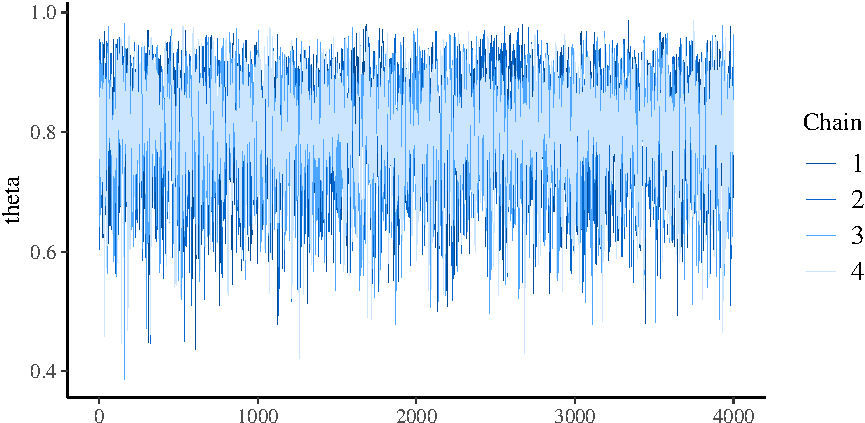
\includegraphics{040_modello_binomiale_files/figure-latex/trace-plot-gautret-1} 

}

\caption{Trace-plot per il parametro $\theta$ nel modello Beta-Binomiale.}\label{fig:trace-plot-gautret}
\end{figure}

\noindent
La figura \ref{fig:trace-plot-gautret} mostra che le catene esplorano uno spazio compreso approssimativamenre tra 0.7 e 0.9; tale figura descrive il comportamento \emph{longitudinale} delle catene di Markov.

Possiamo anche esaminare la distribuzione degli stati della catena di Markov, ovvero, dei valori che queste catene visitano lungo il loro percorso, ignorando l'ordine di queste visite. L'istogramma della figura \ref{fig:hist-post-gautret} fornisce una rappresentazione grafica di questa distribuzione per i 16000 valori complessivi delle quattro catene, ovvero per 4000 valori provienienti da ciascuna catena.

\begin{Shaded}
\begin{Highlighting}[]
\FunctionTok{mcmc\_hist}\NormalTok{(stanfit1, }\AttributeTok{pars =} \StringTok{"theta"}\NormalTok{) }\SpecialCharTok{+}
  \FunctionTok{yaxis\_text}\NormalTok{(}\ConstantTok{TRUE}\NormalTok{) }\SpecialCharTok{+}
  \FunctionTok{ylab}\NormalTok{(}\StringTok{"count"}\NormalTok{)}
\end{Highlighting}
\end{Shaded}

\begin{figure}

{\centering 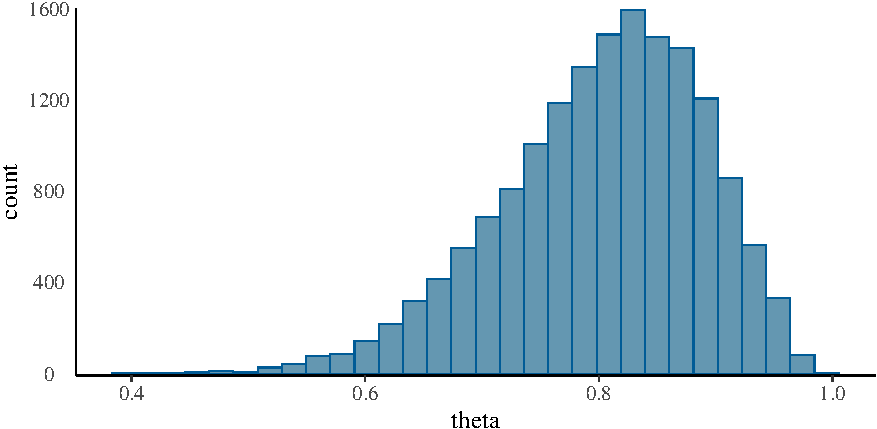
\includegraphics{040_modello_binomiale_files/figure-latex/hist-post-gautret-1} 

}

\caption{Istogramma che illustra l'approssimazione della distribuzione a posteriori per il parametro $\theta$ nel modello Beta-Binomiale.}\label{fig:hist-post-gautret}
\end{figure}

Nel modello Beta-Binomiale in cui la verosimiglianza è binomiale con 14 successi su 16 prove e in cui assumiamo una distribuzione a priori di tipo \(\mbox{Beta}(2, 2)\) sul parametro \(\theta\), la distribuzione a posteriori è ancora una distribuzione Beta di parametri \(\alpha\) = 2 + 14 e \(\beta\) = 2 + 16 - 14. La figura \ref{fig:hist-post-gautret-plus-correct} riporta un kernel density plot per i valori delle quattro catene di Markov con sovrapposta in nero la densità \(\mbox{Beta}(16, 4)\). Il punto importante è che la distribuzione dei valori delle catene di Markov produce un'eccellente approssimazione alla distribuzione bersaglio.\footnote{Nel caso presente, il risultato è poco utile dato che è disponibile una soluzione analitica. Tuttavia, questo esercizio mette in evidenza il fatto cruciale che, nei casi in cui possiamo verificarne la soluzione, il campionamento Monte Carlo a catena di Markov è in grado di trovare la risposta corretta. Di conseguenza, possiamo anche essere sicuri che fornirà un'approssimazione alla distribuzione a posteriori anche in quei casi in cui una soluzione analitica non è disponibile.}

\begin{Shaded}
\begin{Highlighting}[]
\FunctionTok{mcmc\_dens}\NormalTok{(stanfit1, }\AttributeTok{pars =} \StringTok{"theta"}\NormalTok{) }\SpecialCharTok{+}
  \FunctionTok{yaxis\_text}\NormalTok{(}\ConstantTok{TRUE}\NormalTok{) }\SpecialCharTok{+}
  \FunctionTok{ylab}\NormalTok{(}\StringTok{"density"}\NormalTok{) }\SpecialCharTok{+}
  \FunctionTok{stat\_function}\NormalTok{(}\AttributeTok{fun =}\NormalTok{ dbeta, }\AttributeTok{args =} \FunctionTok{list}\NormalTok{(}\AttributeTok{shape1 =} \DecValTok{16}\NormalTok{, }\AttributeTok{shape2 =} \DecValTok{4}\NormalTok{))}
\end{Highlighting}
\end{Shaded}

\begin{figure}

{\centering 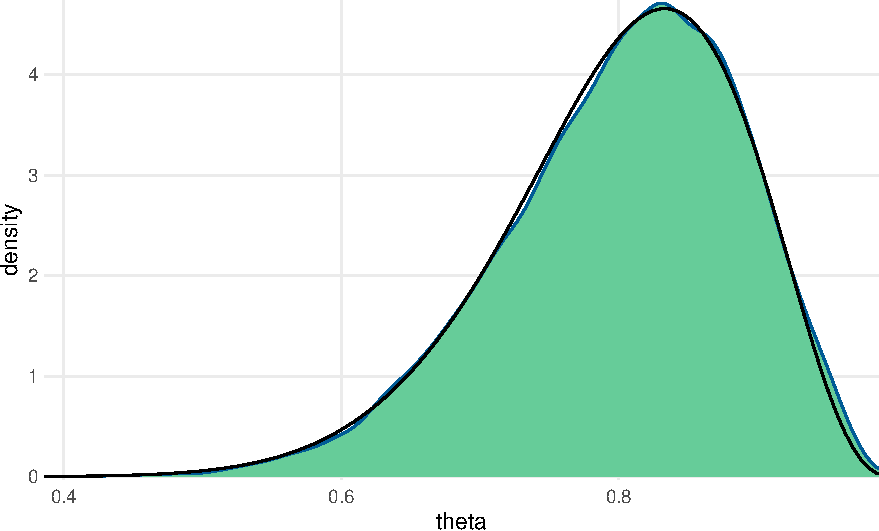
\includegraphics{040_modello_binomiale_files/figure-latex/hist-post-gautret-plus-correct-1} 

}

\caption{Istogramma che illustra l'approssimazione della distribuzione a posteriori per il parametro $\theta$ nel modello Beta-Binomiale. La curva nera rappresenta la corretta distribuzione a posteriori Beta(16, 4).}\label{fig:hist-post-gautret-plus-correct}
\end{figure}

Un intervallo di credibilità al 95\% per \(\theta\) si ottiene con la seguente chiamata:

\begin{Shaded}
\begin{Highlighting}[]
\NormalTok{posterior1 }\OtherTok{\textless{}{-}} \FunctionTok{extract}\NormalTok{(stanfit1)}
\NormalTok{rstantools}\SpecialCharTok{::}\FunctionTok{posterior\_interval}\NormalTok{(}\FunctionTok{as.matrix}\NormalTok{(stanfit1), }\AttributeTok{prob =} \FloatTok{0.95}\NormalTok{)}
\CommentTok{\#\textgreater{}                    2.5\%        97.5\%}
\CommentTok{\#\textgreater{} theta         0.6107860   0.94402990}
\CommentTok{\#\textgreater{} y\_rep[1]      0.0000000   1.00000000}
\CommentTok{\#\textgreater{} y\_rep[2]      0.0000000   1.00000000}
\CommentTok{\#\textgreater{} y\_rep[3]      0.0000000   1.00000000}
\CommentTok{\#\textgreater{} y\_rep[4]      0.0000000   1.00000000}
\CommentTok{\#\textgreater{} y\_rep[5]      0.0000000   1.00000000}
\CommentTok{\#\textgreater{} y\_rep[6]      0.0000000   1.00000000}
\CommentTok{\#\textgreater{} y\_rep[7]      0.0000000   1.00000000}
\CommentTok{\#\textgreater{} y\_rep[8]      0.0000000   1.00000000}
\CommentTok{\#\textgreater{} y\_rep[9]      0.0000000   1.00000000}
\CommentTok{\#\textgreater{} y\_rep[10]     0.0000000   1.00000000}
\CommentTok{\#\textgreater{} y\_rep[11]     0.0000000   1.00000000}
\CommentTok{\#\textgreater{} y\_rep[12]     0.0000000   1.00000000}
\CommentTok{\#\textgreater{} y\_rep[13]     0.0000000   1.00000000}
\CommentTok{\#\textgreater{} y\_rep[14]     0.0000000   1.00000000}
\CommentTok{\#\textgreater{} y\_rep[15]     0.0000000   1.00000000}
\CommentTok{\#\textgreater{} y\_rep[16]     0.0000000   1.00000000}
\CommentTok{\#\textgreater{} log\_lik[1]   {-}0.4930093  {-}0.05759735}
\CommentTok{\#\textgreater{} log\_lik[2]   {-}0.4930093  {-}0.05759735}
\CommentTok{\#\textgreater{} log\_lik[3]   {-}0.4930093  {-}0.05759735}
\CommentTok{\#\textgreater{} log\_lik[4]   {-}0.4930093  {-}0.05759735}
\CommentTok{\#\textgreater{} log\_lik[5]   {-}0.4930093  {-}0.05759735}
\CommentTok{\#\textgreater{} log\_lik[6]   {-}0.4930093  {-}0.05759735}
\CommentTok{\#\textgreater{} log\_lik[7]   {-}0.4930093  {-}0.05759735}
\CommentTok{\#\textgreater{} log\_lik[8]   {-}0.4930093  {-}0.05759735}
\CommentTok{\#\textgreater{} log\_lik[9]   {-}0.4930093  {-}0.05759735}
\CommentTok{\#\textgreater{} log\_lik[10]  {-}0.4930093  {-}0.05759735}
\CommentTok{\#\textgreater{} log\_lik[11]  {-}0.4930093  {-}0.05759735}
\CommentTok{\#\textgreater{} log\_lik[12]  {-}0.4930093  {-}0.05759735}
\CommentTok{\#\textgreater{} log\_lik[13]  {-}0.4930093  {-}0.05759735}
\CommentTok{\#\textgreater{} log\_lik[14]  {-}0.4930093  {-}0.05759735}
\CommentTok{\#\textgreater{} log\_lik[15]  {-}2.8829362  {-}0.94362543}
\CommentTok{\#\textgreater{} log\_lik[16]  {-}2.8829362  {-}0.94362543}
\CommentTok{\#\textgreater{} lp\_\_        {-}12.7342100 {-}10.00860000}
\end{Highlighting}
\end{Shaded}

Svolgendo un'analisi bayesiana simile a questa, \citet{Gautret_2020} hanno trovato che gli intervalli di credibilità del gruppo di controllo e del gruppo sperimentale non si sovrappongono. Questo fatto viene interpretato dicendo che il parametro \(\theta\) è diverso nei due gruppi. Sulla base di queste evidenza, \citet{Gautret_2020} hanno concluso, con un grado di certezza soggettiva del 95\%, che nel gruppo sperimentale vi è una probabilità più bassa di risultare positivi al SARS-CoV-2 rispetto al gruppo di controllo. In altri termini, questa analisi dei dati suggerisce che l'idrossiclorochina sia efficace come terapia per il Covid-19.

\hypertarget{la-critica-di-hulme_2020}{%
\subsection{\texorpdfstring{La critica di \citet{Hulme_2020}}{La critica di @Hulme\_2020}}\label{la-critica-di-hulme_2020}}

Un articolo pubblicato da \citet{Hulme_2020} si è posto il problema di rianalizzare i dati di \citet{Gautret_2020}.\footnote{Si veda \url{https://osf.io/5dgmx/}.} Tra gli autori di questo articolo figura anche Eric-Jan Wagenmakers, uno psicologo molto conosciuto per i suoi contributi metodologici.
\citet{Hulme_2020} hanno osservato che, nelle analisi statistiche riportate, \citet{Gautret_2020} hanno escluso alcuni dati. Nel gruppo sperimentale, infatti, vi erano alcuni pazienti i quali, anziché migliorare, sono in realtà peggiorati. L'analisi statistica di \citet{Gautret_2020} ha escluso i dati di questi pazienti.
Se consideriamo tutti i pazienti --- non solo quelli selezionati da \citet{Gautret_2020} --- la situazione diventa la seguente:

\begin{itemize}
\tightlist
\item
  gruppo sperimentale: 10 positivi su 18;
\item
  gruppo di controllo: 14 positivi su 16.
\end{itemize}

L'analisi dei dati proposta da \citet{Hulme_2020} richiede l'uso di alcuni strumenti statistici che, in queste dispense, non verranno discussi. Ma possiamo giungere alle stesse conclusioni raggiunte da questi ricercatori anche usando le procedure statistiche descritte nel Paragrafo successivo.

\hypertarget{due-proporzioni}{%
\section{Due proporzioni}\label{due-proporzioni}}

Svolgiamo ora l'analisi considerando tutti i dati, come suggerito da \citet{Hulme_2020}. Per fare questo verrà creato un modello bayesiano per fare inferenza sulla differenza tra due proporzioni. Una volta generate le distribuzioni a posteriori per le proporzioni di ``successi'' nei due gruppi, verrà anche generata la quantità
\[
\omega = \frac{\theta_2 / (1-\theta_2)}{\theta_1 / (1-\theta_1)},
\]
\noindent
ovvero il rapporto tra gli Odds di positività tra i pazienti del gruppo di controllo e gli Odds di positività tra i pazienti del gruppo sperimentale. Se il valore dell'OR è uguale a 1, significa che l'Odds di positività nel gruppo di controllo è uguale all'odds di positività nel gruppo sperimentale, cioè il fattore in esame (somministrazione dell'idrossiclorochina) è ininfluente sulla comparsa della malattia. L'inferenza statistica sull'efficacia dell'idrossiclorochina come terapia per il Covid-19 può dunque essere effettuata esaminando l'intervallo di credibilità al 95\% per l'OR: se tale intervallo include il valore 1, allora non vi è evidenza che l'idrossiclorochina sia efficace come terapia per il Covid-19.

Nell'implementazione di questo modello, la quantità di interesse è dunque l'odds ratio; tale quantità viene calcolata nel blocco \texttt{generated\ quantities} del programma Stan. In questo esempio useremo delle distribuzioni a priori vagamente informative per i parametri \(\theta_1\) e \(\theta_1\).

\begin{Shaded}
\begin{Highlighting}[]
\NormalTok{data\_list }\OtherTok{\textless{}{-}} \FunctionTok{list}\NormalTok{(}
  \AttributeTok{N1 =} \DecValTok{18}\NormalTok{,}
  \AttributeTok{y1 =} \DecValTok{10}\NormalTok{,}
  \AttributeTok{N2 =} \DecValTok{16}\NormalTok{,}
  \AttributeTok{y2 =} \DecValTok{14}
\NormalTok{)}
\end{Highlighting}
\end{Shaded}

\begin{Shaded}
\begin{Highlighting}[]
\NormalTok{modelString }\OtherTok{\textless{}{-}} \StringTok{"}
\StringTok{//  Comparison of two groups with Binomial}
\StringTok{data \{}
\StringTok{  int\textless{}lower=0\textgreater{} N1;              // number of experiments in group 1}
\StringTok{  int\textless{}lower=0\textgreater{} y1;              // number of deaths in group 1}
\StringTok{  int\textless{}lower=0\textgreater{} N2;              // number of experiments in group 2}
\StringTok{  int\textless{}lower=0\textgreater{} y2;              // number of deaths in group 2}
\StringTok{\}}
\StringTok{parameters \{}
\StringTok{  real\textless{}lower=0,upper=1\textgreater{} theta1; // probability of death in group 1}
\StringTok{  real\textless{}lower=0,upper=1\textgreater{} theta2; // probability of death in group 2}
\StringTok{\}}
\StringTok{model \{}
\StringTok{  theta1 \textasciitilde{} beta(2, 2);          // prior}
\StringTok{  theta2 \textasciitilde{} beta(2, 2);          // prior}
\StringTok{  y1 \textasciitilde{} binomial(N1, theta1);    // observation model / likelihood}
\StringTok{  y2 \textasciitilde{} binomial(N2, theta2);    // observation model / likelihood}
\StringTok{\}}
\StringTok{generated quantities \{}
\StringTok{  // generated quantities are computed after sampling}
\StringTok{  real oddsratio = (theta2/(1{-}theta2))/(theta1/(1{-}theta1));}
\StringTok{\}}
\StringTok{"}
\FunctionTok{writeLines}\NormalTok{(modelString, }\AttributeTok{con =} \StringTok{"code/twoprop1.stan"}\NormalTok{)}
\end{Highlighting}
\end{Shaded}

\begin{Shaded}
\begin{Highlighting}[]
\NormalTok{file }\OtherTok{\textless{}{-}} \FunctionTok{file.path}\NormalTok{(}\StringTok{"code"}\NormalTok{, }\StringTok{"twoprop1.stan"}\NormalTok{)}
\end{Highlighting}
\end{Shaded}

\begin{Shaded}
\begin{Highlighting}[]
\NormalTok{mod }\OtherTok{\textless{}{-}} \FunctionTok{cmdstan\_model}\NormalTok{(file)}
\end{Highlighting}
\end{Shaded}

\begin{Shaded}
\begin{Highlighting}[]
\NormalTok{fit }\OtherTok{\textless{}{-}}\NormalTok{ mod}\SpecialCharTok{$}\FunctionTok{sample}\NormalTok{(}
  \AttributeTok{data =}\NormalTok{ data\_list,}
  \AttributeTok{iter\_sampling =}\NormalTok{ 4000L,}
  \AttributeTok{iter\_warmup =}\NormalTok{ 2000L,}
  \AttributeTok{seed =}\NormalTok{ SEED,}
  \AttributeTok{chains =}\NormalTok{ 4L,}
  \AttributeTok{parallel\_chains =}\NormalTok{ 4L,}
  \AttributeTok{refresh =} \DecValTok{0}\NormalTok{,}
  \AttributeTok{thin =} \DecValTok{1}
\NormalTok{)}
\end{Highlighting}
\end{Shaded}

\begin{Shaded}
\begin{Highlighting}[]
\NormalTok{stanfit }\OtherTok{\textless{}{-}}\NormalTok{ rstan}\SpecialCharTok{::}\FunctionTok{read\_stan\_csv}\NormalTok{(fit}\SpecialCharTok{$}\FunctionTok{output\_files}\NormalTok{())}
\end{Highlighting}
\end{Shaded}

\begin{Shaded}
\begin{Highlighting}[]
\FunctionTok{print}\NormalTok{(}
\NormalTok{  stanfit,}
  \AttributeTok{pars =} \FunctionTok{c}\NormalTok{(}\StringTok{"theta1"}\NormalTok{, }\StringTok{"theta2"}\NormalTok{, }\StringTok{"oddsratio"}\NormalTok{),}
  \AttributeTok{digits\_summary =}\NormalTok{ 3L}
\NormalTok{)}
\CommentTok{\#\textgreater{} Inference for Stan model: twoprop1{-}202110101000{-}1{-}60e488.}
\CommentTok{\#\textgreater{} 4 chains, each with iter=6000; warmup=2000; thin=1; }
\CommentTok{\#\textgreater{} post{-}warmup draws per chain=4000, total post{-}warmup draws=16000.}
\CommentTok{\#\textgreater{} }
\CommentTok{\#\textgreater{}            mean se\_mean    sd  2.5\%   25\%   50\%   75\%}
\CommentTok{\#\textgreater{} theta1    0.546   0.001 0.104 0.337 0.475 0.547 0.619}
\CommentTok{\#\textgreater{} theta2    0.801   0.001 0.087 0.605 0.747 0.812 0.865}
\CommentTok{\#\textgreater{} oddsratio 4.859   0.049 4.740 0.914 2.221 3.599 5.933}
\CommentTok{\#\textgreater{}            97.5\% n\_eff  Rhat}
\CommentTok{\#\textgreater{} theta1     0.743 11214 1.000}
\CommentTok{\#\textgreater{} theta2     0.939 12359 1.000}
\CommentTok{\#\textgreater{} oddsratio 16.251  9207 1.001}
\CommentTok{\#\textgreater{} }
\CommentTok{\#\textgreater{} Samples were drawn using NUTS(diag\_e) at Dom Ott 10 10:00:03 2021.}
\CommentTok{\#\textgreater{} For each parameter, n\_eff is a crude measure of effective sample size,}
\CommentTok{\#\textgreater{} and Rhat is the potential scale reduction factor on split chains (at }
\CommentTok{\#\textgreater{} convergence, Rhat=1).}
\end{Highlighting}
\end{Shaded}

L'intervallo di credibilità del 95\% per l'OR include il valore di 1.0 (ovvero, il valore che indica che gli odds di positività sono uguali nei due gruppi). In base agli standard correnti, un risultato di questo tipo non viene considerato come evidenza sufficiente per potere concludere che il parametro \(\theta\) assume un valore diverso nei due gruppi. In altri termini, se consideriamo tutti i dati, e non solo quelli selezionati dagli autori della ricerca originaria, non vi è evidenza alcuna che l'idrossiclorochina sia efficace come terapia per il Covid-19.

\hypertarget{considerazioni-conclusive}{%
\section*{Considerazioni conclusive}\label{considerazioni-conclusive}}
\addcontentsline{toc}{section}{Considerazioni conclusive}

Concludiamo questa discussione dicendo che ciò che è stato presentato in questo capitolo è un esercizio didattico: la ricerca di \citet{Gautret_2020} include tante altre informazioni che non sono state qui considerate. Tuttavia, notiamo che la semplice analisi statistica che abbiamo qui descritto è stata in grado di replicare le conclusioni a cui sono giunti (per altra via) \citet{Hulme_2020}.

  \bibliography{refs.bib,book.bib,packages.bib}

\end{document}
